% !TEX encoding = UTF-8 Unicode
\documentclass[12pt,a4paper]{article}
\usepackage[ngerman]{babel}
\usepackage[utf8]{inputenc}
\usepackage[T1]{fontenc}
\usepackage{lmodern}
\usepackage{graphicx}
\usepackage{enumerate}
\usepackage[]{epstopdf}
\usepackage[margin=1in]{geometry}
\usepackage{titling}
\usepackage{hyperref}
\usepackage[german]{cleveref}
\usepackage{amsmath,amsthm,verbatim,amssymb,amsfonts,amscd}
\usepackage{braket}
\renewcommand{\familydefault}{\sfdefault}
\usepackage[miktex]{gnuplottex}
\usepackage[decimalsymbol=comma,separate-uncertainty=true,expproduct=\cdot,
            uncertainty-separator=\pm]{siunitx}
\setlength{\droptitle}{-2cm}
\title{Auswertung zu IQ13:\\
       magneto-optische Falle\\
       WiSe 15/16\\
       Block III}
\author{Ramin Javadi 2993630 und Felix Schrader 3053850}
\date{}
\begin{document}
\maketitle
\tableofcontents
\pagebreak
\section{Theorie einer MOT}
  \subsection{Optische Melasse}
  
  Laserkühlung von Atomen, das ist die Reduktion der atomaren Geschwindigkeitsverteilung durch in diesem Fall Laserlicht, dabei spielt der Strahlungsdruck wichtige Rolle, der zur Spontankraft führt. In einer Dimension betrachten wir die Wechselwirkung eines Lasers mit einem Zwei-Niveau-Atom mit der Übergangsfrequenz ${\omega_A}$. Wenn ein Laser ${\omega_A}$ rotverstimmt ist und ein entgegenkommende Atom einer Geschwindigkeit ${\vec v}$ hat, wird dieses Atom Photonen absorbieren aufgrund des Dopplereffekts, danach wird aus dem Laserstrahl das Photon spontan und somit ohne Richtung emittiert.
  
  Findet bei jedem Absorptions- und Emissionsprozeß ein Impulsübertrag statt. Wenn aus einer Richtung die Absorption passiert, ist die spontane Emission ungerichtet und auch die Impulsänderung durch sie im Mitte null. Deswegen wird ein Gesamtimpuls in Richtung des Laserstrahles auf das Atom übertragen.
 \\Auf das Atom durch die absorption wirkt eine Kraft, sie lässt sich als Produkt aus Impulsübertrag ${\hbar \vec k \Gamma}$, wobei ${\Gamma}$ der Streurate der Photonen ist: 
   \begin{align*}
  \vec F=\hbar \vec k \Gamma
  \end{align*}
  Diese Spontankraft ist zum Abbremsen (Kühlen) von Atomen. wenn man Intensität des Lasers ${I}$ höher macht, wird Streurate größer, und sie hängt auch von der Verstimmung des Lasers ${\delta_L}$ . Dabei entspricht ${\Gamma =1/ \tau}$, ${\tau}$ ist Lebensdauer des angeregten Zustands.
  \\Diese Verstimmung kann man erstens durch Differenz von Frequenz des Lasers ${\omega_A}$ und die atomare Übergasfrequenz ${\omega_A}$ und zweitens aus der Dopplerverstimmung ${\vec k \vec v}$ bestimmen.
   \begin{align*}
    \vec F=\frac{\hbar \vec k}{2 \tau} \frac{I/I_0}{1+I/I_0+(\frac{ \delta _L-\vec k \vec v}{\Gamma /2})^2}
  \end{align*}
  Wie in Abbildung \ref{fvonv} zu sehen, ist die Ausbreitungsrichtung des Atoms in -z-Richting, eine positive Kraft und in +z-Richtung, eine negative Kraft wird ausgeübt und in beiden Fällen auf eine Geschwindigkeit ${v\approx 0}$ werden abgebremst. Ist eine Geschwindigkeitsdämpfung möglich, im Bereich, wo die Kraft auf ein Atom sich linear ändert.
   \begin{figure}[h!]
  \centering
  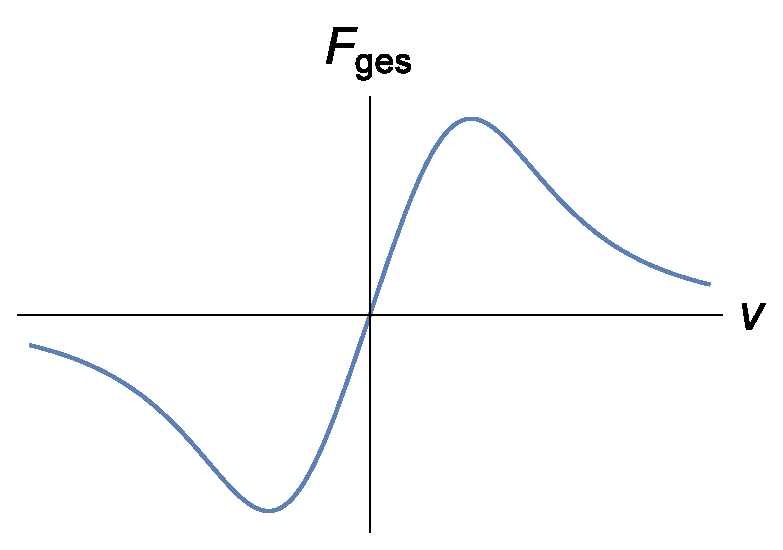
\includegraphics[width=0.6\textwidth]{fvonv.eps}
  \caption{F von v}
  \label{fvonv}
  \end{figure}
  Unter Optische Melasse versteht man dieser Geometrie auf drei Dimensionen von Laserstrahlen, indem drei senkrecht zueinander stehende Laser, die jeweils in sich zurückreflektiert werden und dadurch bewirken die räumliche Kühlung von Atomen.
 \\In einer Optische Melasse ist die Temperatur ${T}$ im Gleichgewicht zwischen der Kühlrate durch Absorption und Heizrate durch stochastischen Charakter der Emissionen.
 \\Durch Optische Melasse werden die Atome im Impulsraum gefangen. Eine Einschränkung im Ortsraum ist mit dieser Anordnung jedoch nicht möglich, deswegen eine optische Melasse ist keine echte Falle. Die Atome bewegen sich wie in einer viskosen Flüssigkeit. 
 
 Die Einschränkung im Ortsraum kann zusätzliches Quadrupo-Magnetfeld erreicht werden. Diese Idee ist Grundlage zur Theorie der magnetooptischen Falle.
  \subsection{Magnetfeld}
  Zunächst betrachten wir ein Zwei-Niveau-Atom in einer Dimension mit einem Grundzustand ${J=0}$ und einem angeregten Zustand ${J=1}$. 
  \\Ein Quadrupol-Magnetfeld ${\vec B}$ wird erzeugt, um eine Ortsabhängigkeit der Resonanzfrequenz ${\omega_0}$ zu kriegen, was auch zu einer Aufspaltung des angeregten Zustands in drei Zeeman-Unterzustände führt (${m_J=-1,0,1}$), wegen Zeeman-Effekts.
  
  Was wir hier betrachten ist eine Anordnung Zwei zirkular polarisierte Laser, die auch entgegengesetzt auf Atome eingestrahlt werden. Der rechte Laser ist linkszirkular polarisiert und der linke Laser rechtszirkular polarisiert. Dabei sind beide Laser rotverstimmt.
  \\Solange ein Atom sich nicht bewegt bzw. in Fallenzentrum befindet, wirkt keine Kraft. Bewegt sich das Atom z.B. nach links, so absorbiert mit hoher Wahrscheinlichkeit ein Photon aus dem ${\sigma^+}$-Strahl, weil es mit diesem rotverstimmten Laser in Resonanz kommt und das Atom wird Angeregt und bekommt den Zustand $\ket{J=1 , m_J=+1}$ . 
  \\Das Atom erfährt eine Kraft durch die Streuung der Photonen an dem Atom, die auch dazu führt , daß das Atom ins Fallenzentrum zurückkehrt. Die Absorption eines Photons aus dem ${\sigma^-}$ -Strahl passiert sehr Unwahrscheinlich. Analog passiert für das Atom, wenn es nach rechts aus dem Fallenzentrum bewegt. 
  \begin{figure}[h!]
  \centering
  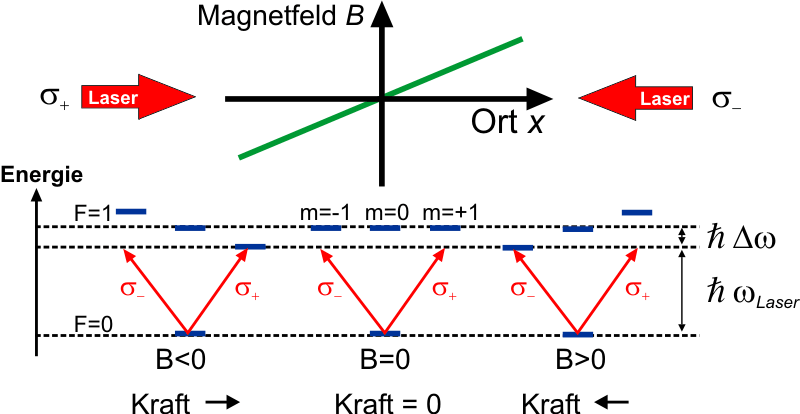
\includegraphics[width=0.6\textwidth]{Mot_posforce.png}
  \caption{die Aufspaltung des angeregten Zustands durch den Zeeman-Effekt und die ortsabhängige Kraft (Quelle: \detokenize{https://de.wikipedia.org/wiki/Magneto-optische_Falle})}
  \label{zeemanmot}
  \end{figure}\\
 Mit dieser Überlegung erreicht man eine räumliche Begrenzung der Atome. Im dreidimensionalen Fall wird ein Quadrupol-Magnetfeld durch zwei gegensinnig durch- flossene Spulen erreicht. Das Magnetfeld verläuft in einer Umgebung des Fallenzentrums linear, so daß eine Aufspaltung des angeregten Zustands, wie in Abbildung \ref{zeemanmot}, erreicht wird.
  \subsection{Übergänge von ${}^{87}$Rb}
  Ausgewähltes Element für das versuch war Rubidium. Zur Laserkühlung ist Rubidium aus verschiedenen Gründen gut geeignet. Erstens gibt es kostengünstige und kompakte Diodenlaser mit einer ähnlichen Frequenz wie der des Kühlübergangs von Rubidium, zweitens hat das Element einen hohen Dampfdruck von ${10^{-8}}$ Torr bei 300K. Deswegen muss man die Atome nicht stark erhitzen, ist es nicht nötig, wie es z.B. bei Natrium der Fall ist.
${}^{87}$Rb ist ein Alkalimetall mit einem Elektron in der äußersten, der vierten Schale. Im Grundzustand 5S1/2 besitzt das Atom einen Drehimpuls
   ${|J = 1/2>}$ und im ersten angeregten Zustand $5P_{3/2}$ einen Drehimpuls${ |J = 3/2>}$ . Der Drehimpulsvektor I des Protons beträgt bei ${}^{87}$Rb $I$ = 5/2. Es ergibt sich ein Gesamtdrehimpuls. Für den Grundzustand ergeben sich folglich F = 2 und F = 3, sowie F'= 1,...,4 für den ersten angeregten Zustand.
Für eine MOT mit Rb-Atomen benötigt man folglich zwei Laser, die bei leicht unterschiedlichen Frequenzen (Frequenzabstand ${\Delta}$ = 2.9 GHz) laufen. Um die Laser auf der richtigen Frequenz zu betreiben, werden diese sättigungsspektroskopisch stabilisiert. $\rightarrow$
\section{Bestandteile der MOT}
  \subsection{Die Laser}
    In dem Versuchsaufbau werden zwei Halbleiterlaser (Kühl- und Rückpumplaser)
    verwendet. Der Kühllaser wird mit ca. \SI{85}{\mA}, der Rückpumper mit ca.
    \SI{160}{\mA} betrieben. Durch Anlegen eines Stromes in Durchlassrichtung
    einer p-n-Diode entsteht eine dünne Schicht, in der es eine Besetzungsinversion
    mit Löchern im Valenz- und Elektronen im Leitungsband gibt. Als Resonator
    dienen die Stirnflächen der Diode. Durch Änderung des Stromes kann man die
    emittierte Wellenlänge ändern, allerdings erhöht sich gleichzeitig die
    Laserleistung. Ein Problem der Laser ist, dass sich durch leichte
    Temperaturänderungen die optische Weglänge des Lasers ändert und es somit zu
    Modensprüngen kommt. Um diese zu umgehen (und zum feineren Einstellen der
    Wellenlänge) wird ein Gitter als externe Cavity verwendet. Die erste
    Beugungsordnung wird dabei zurückreflektiert. Der Winkel, unter dem der Strahl
    von Gitter reflektiert wird ist von der Wellenlänge abhängig, daher kann man
    durch drehen des Gitters eine Änderung der Wellenlänge erreichen. Um das Gitter
    zu drehen ist es auf einem Piezo-Kristall befestigt. Durch Änderung des Stromes
    am Piezo-Element, ändert sich dessen Temperatur und damit dessen Ausdehnung, das
    Gitter wird also bewegt. Die Reflexion in die nullte Ordnung wird als Laserlicht
    verwendet. Um Rückreflexe in die Diode zu verhindern steht hinter den Lasern
    jeweils ein Isolator.
  \subsection{Laserlocken}
    Um die Laser zu koppeln wird ein kleiner Teil des Lichts in den
    Spektroskopiepfad ausgekoppelt. Dort befindet sich ein Aufbau zur
    Sättigungsspektroskopie. Dabei wird der Strahl durch eine Glasscheibe geschickt
    (es entstehen zwei Reflexe, einer an der Vorder- einer an der Rückseite der
    Scheibe) und über einen Spiegel in eine Rubidiumzelle geleitet (Pumpstrahl). Die
    beiden Reflexe von der Glasplatte werden ebenfalls in die Rubidiumzelle geschickt,
    allerdings von der anderen Seite (dadurch sind sie jeweils in die andere Richtung
    dopplerverschoben, wie der Pumpstrahl). Dabei passiert der stärkere Reflex
    (Abfragestrahl) in der Zelle einen Bereich, den auch der Pumpstrahl durchläuft.
    Beide brennen dadurch Löcher in das normale Dopplerprofil, die im gleichen
    Abstand links und rechts vom Maximum sind. Stellt man die Wellenlänge richtig ein,
    können sich beide Löcher im Profil überlagern (die Rubidiumatome können also von
    beiden Strahlen angeregt werden). Dies kann passieren, wenn man genau auf
    Resonanz mit einem Übergang ist (da beide Strahlen um den gleichen Betrag
    dopplerverschoben sind ist Absorption von Licht aus beiden Strahlen gleich
    wahrscheinlich $\rightarrow$ Lamb-Dip) oder wenn die Wellenlänge genau zwischen
    zwei Übergängen liegt (beide Strahlen regen jeweils unterschiedliche Übergänge an
    $\rightarrow$ Cross-Over-Resonanz). Da auf dem Oszilloskop die Absorption des
    Laserlichts angezeigt wird, erscheinen diese Dips als kleine Maxima im
    Dopplerprofil. Der schwächere Reflex von der Glasplatte durchläuft die
    Rubidiumzelle an einer anderen Stelle und misst somit zum Vergleich das reine
    Dopplerprofil.
    
    Um die Laser zu locken wird der Strom am Piezoelement so eingestellt, dass man
    genau den gewünschten Lamb-Dip erhält. Dabei wird auf dem Oszilloskop das
    Signal vom Abfragestrahl (mit Dopplerprofil) angezeigt, zum Locken wird die
    Differenz von Abfragestrahl und Dopplerprofil verwendet. Leichte Änderungen der
    Wellenlänge (z.B. durch wackeln der Cavity oder Temperaturänderungen) sorgen
    dafür, dass das Signal nicht mehr auf einem Maximum ist. Dann wird der Strom
    automatisch auf den richtigen Wert geregelt um wieder das Maximum zu erreichen.
    Da allerdings nicht klar ist, auf welcher Seite vom Maximum man sich befindet
    wird das Signal zunächst abgeleitet. Die Ableitung des Signals erfolgt durch
    Modulierung des Stromes mit einer Sinuskurve. Dies erlaubt Messungen auf beiden
    Seiten leicht neben dem betrachteten Punkt und somit eine Abschätzung der Steigung
    also eine Ableitung. Das Locken erfolgt dann auf einem Nulldurchgang der Ableitung.
  \subsection{Der AOM}
    
  \subsection{Der TA}
  \subsection{Die Vakuumkammer}
  \subsection{Die Kamera}
\section{Messungen}
  \subsection{Intensitätsmessungen im Strahlengang}
  \subsection{Vermessung der Strahlbreite}
  \subsection{Eichung der Kamera}
\end{document}